\documentclass[a4paper,oneside,12pt]{report}

\usepackage{../custom}

\usepackage[backend=biber]{biblatex}
\addbibresource{biblio.bib}

\begin{document}

\begin{titlepage}
    \begin{center}
        \vspace*{1cm}
        
        \Huge
	\textbf{Procédé de production d'ammoniac}
        
        \vspace{1cm}
        
        \textbf{Groupe 1225}
        
        \vspace{0.5cm}
        
        \large
        Un rapport réalisé dans le cadre du cours\\
        
        \LARGE
        Projet Q3 - LFSAB1503
        \vspace{0,5cm}
        
        %\includegraphics[scale = 0.25]{img/divers/coverpicture.png}        
        %\vfill
        
        %\includegraphics[scale = 0.2]{img/divers/epl-logo.jpg}
        %\vspace{1cm}

        \vfill 
        \large
        
	de Bellefroid Cédric ($32631100$) \\
	Dénos Cyril ($62811300$) \\
        de Wasseige John ($52241300$) \\
	Dispas David ($71891200$) \\
	Libeer Cassian  ($65161200$) \\
        Malengreau Tim ($66081300$) \\
	Paquet Arnaud ($36681300$) \\       
        
    \end{center}
\end{titlepage}


\tableofcontents

\chapter{Introduction}
%\input{intro}
\chapter{Page de synthèse}
%\input{syntese}

\appendix
\chapter{Rapports précédents}

\section{T\^ache 1}
%\documentclass[a4paper, oneside, 12pt]{article}

\usepackage{../custom}

\title{Rapport 1}
\author{Groupe 1225}
\date{\today}

\begin{document}

\maketitle

\section{Bilan de matière}

Nous faisons l'hypothèse que la réaction est parfaite, 
c'est-à-dire que tous les réactifs sont consommés 
et que l'on obtient uniquement le produit.

Il faut déterminer la quantité de dihydrogène (\ce{H2}) et d'azote (\ce{N2}) 
nécéssaire pour produire $1000 \si{\tonne}$ d'ammoniac (\ce{NH3}).

\begin{equation}
	\ce{\frac{3}{2} \, H2 + \frac{1}{2} \, N2 -> NH3} 
	\label{eq:ammoniac}
\end{equation}

La masse molaire de l'ammoniac vaut $17 \si{\gram\per\mole}$,
il faut donc en produire $5.88\e{7} \si{\mole}.$

On obtient les nombres de moles de réactifs à partir de la réaction pondérée. 

\begin{align*}
	m_{\ce{H2}}  = \frac{3}{2} \, n_{\ce{NH3}} \cdot M_{m, \ce{H2}} 
	= 1.765\e{8} \si{\gram} \\
	m_{\ce{N2}} = \frac{1}{2} \, n_{\ce{NH3}} \cdot M_{m, \ce{N2}} 
	= 8.235\e{8} \si{\gram}
\end{align*}

Les masses de \ce{H2} et de \ce{N2} valent donc 
respectivement $176.5 \si{\tonne}$ et $823.5 \si{\tonne}$.
Le bilan de masse est correct : si on fait la somme des masses des réactifs,
on retrouve la même masse produite.


\section{Débit d'eau nécessaire}

Afin de maintenir les réacteurs à température constante, 
on refroidit ceux-ci avec de l'eau.
Il faut tout d'abord calculer la chaleur dégagée par jour par les réacteurs,
pour ensuite déterminer la quantité d'eau nécessaire pour absorber cette chaleur,
sachant que l'eau entre à $25 \si{\degreeCelsius}$ et 
est évacuée à $90 \si{\degreeCelsius}$. 

\paragraph{In}

La chaleur dégagée par la réaction \ref{eq:ammoniac} correspond à la 
différence entre l'enthalpie de formation des produits et celle des réactifs. 

\begin{equation}
	\Delta H_{reaction} = \Delta H_{f, \ce{NH3}} 
	- \frac{1}{2} \Delta H_{f, \ce{N2}}
	- \frac{3}{2} \Delta H_{f, \ce{H2}}
	\label{eq:enthalpie_reaction}
\end{equation}

La réaction se passe à $500 \si{\degreeCelsius}$, 
on détermine donc les $\Delta H_{f}$ des différents 
composés à partir des valeurs des enthalpies standard
de formation\footnote{Atkins \& Jones - Chemical Principles}
(à $25 \si{\degreeCelsius}$)
et des capacités calorifiques molaires ($C_p$), gr\^ace 
à l'équation suivante.

\begin{equation*}
	\Delta H_{f, T2} = \Delta H_{f, T1} 
	+ \int_{T1}^{T2} C_p \, \dif{T}
\end{equation*}

Étant donné que nous travaillons avec des quantités importantes de matière,
nous ne pouvons pas considérer que $C_p$ est constant.
On sait que $C_p$ varie en fonction de la température 
selon une fonction $a + b T + c T^2$, 
où $a$, $b$ et $c$ sont des constantes\footnote{\url{http://www.edu.upmc.fr/
chimie/lc101-202-301/communs/public/capcalo.htm}}. 

Nous pouvons à présent calculer les enthalpies 
de formation à $500 \si{\degreeCelsius}$

\begin{equation}
	\Delta H_f = \Delta H_{f}^{\si{\degree}} + 
	\int_{298}^{773} (a + b T + c T^2) \, \dif{T}
	\label{eq:enthalpie_500C}
\end{equation}

À partir de l'équation \ref{eq:enthalpie_500C}, 
on obtient les valeurs suivantes

\begin{align*}
	\Delta H_{\ce{H2}} &= 14 \, \si{\kilo\joule\per\mole} \\
	\Delta H_{\ce{N2}} &= 14.19 \, \si{\kilo\joule\per\mole} \\
	\Delta H_{\ce{NH3}} &= -26.21 \, \si{\kilo\joule\per\mole} 
\end{align*}

Pour finir, on trouve l'enthalpie de réaction par l'équation \ref{eq:enthalpie_reaction}

\[
	\Delta H_{reaction} = -54.31 \, \si{\kilo\joule\per\mole}
\]

\paragraph{Out}

Le raisonnement pour la chaleur absorbée est similaire 
au précédent, sauf que cette fois ci, 
on considère que la capacité calorifique est constante.
Cette hypothèse peut être raisonnablement envisagée 
étant donné que\footnote{\url{http://kinetics.nist.gov/janaf/html/H-065.html}} 
$C_{p, 298 \si{\kelvin}} \approx 75.35 \, \si{\joule\per\kelvin\per\mole}$ 
et $C_{p, 368 \si{\kelvin}} \approx 75.78 \, \si{\joule\per\kelvin\per\mole}$.
La différence étant très petite, 
nous prendrons la moyenne de ces deux valeurs. 

La chaleur absorbée par une mole d'eau vaut exactement

\begin{equation}
	\Delta H = \int_{298}^{363} C_{p, \ce{H2O}} \, \dif{T}
	= 75.565 \cdot 65 = 4911.73 \, \si{\joule\per\mole}
\end{equation}

\paragraph{Débit}

Il s'agit maintenant de déterminer la quantité d'eau nécessaire par jour.
Il faut que

\[
	\frac{\Delta H_{in}}{\mathrm{jour}} 
	= - \frac{\Delta H_{out}}{\mathrm{jour}}
\]

En sachant qu'on produit $1000 \si{\tonne}$ de \ce{NH3} par jour
(cela équivaut à $5.88\e{7} \, \si{\mole}$),
et à partir des données trouvées ci-dessus, 
on trouve que

\begin{align*}
	n_{\ce{H2O}} &= \frac{n_{\ce{NH3}} \, \Delta H_{in}}{\Delta H_{out}} \\
	&= 6.5\e{8} \si{\mole} 
\end{align*}

Il faut donc $11703 \si{\tonne}$ d'eau par jour, 
ou encore 136 litres par seconde.

\end{document}



\section{T\^acihe 2}
%\documentclass[a4paper, oneside, 12pt]{article}

\usepackage{../custom}

\usepackage[backend=biber]{biblatex}
\addbibresource{biblio.bib}

\title{Tâche 2}
\author{Groupe 1225}
\date{\today}

\begin{document}

\maketitle

\section{Analyse des conditions optimales du réacteur de synthèse d'ammoniac}

Jusqu'ici nous avons considéré la dernière étape du procédé - la synthèse d'ammoniac -
comme une bo\^ite noire. Nous allons maintenant déterminer quelles sont les conditions 
optimales de température et de pression pour ce réacteur. 
Avant de commencer, il nous semble important de rappeler le principe 
de \textsc{Le Ch\^atelier} : \enquote{Si l'on tend à modifier les conditions d'un système en équilibre, 
il réagit de façon à s'opposer, en partie, aux changements qu'on lui impose, 
jusqu'à l'établissement d'un nouvel équilibre.}. \cite{chatelier}

La réaction de synthèse l'ammoniac est la suivante
\[\ce{N2_{(g)} + 3H2_{(g)} <=> 2NH3_{(g)} } \]

\paragraph{Pression}

On voit tout de suite que le nombre de moles de gaz de réactifs est supérieur 
au nombre de moles de gaz des produits, 
plus précisément $n_{g}\text{(réactifs)} = 2 \cdot n_{g}\text{(produits)}$.

Par la loi des gaz parfait, on sait que la pression est directement proportionnelle 
au nombre de moles de gaz. Le principe énoncé ci-dessus
nous permet de dire qu'une \emph{augmentation} de la pression du réacteur ($p_{\text{total}}$),
favorisera le sens de la diminution du nombre de moles de gazs, 
et dans notre cas, favorisera la production de \ce{NH3}.

\[
K = \frac{p_{eq,\ce{NH3}}^2}{p_{eq,\ce{H2}}^3 \cdot p_{eq,\ce{N2}} \cdot p_{\text{total}}^2}
\]
\paragraph{Température}

La réaction de synthèse est une réaction fortement exothermique 
(à $700\si{\kelvin}$, $\Delta_r H^{\circ} = -52.6\si{\kilo\joule}$).
Pour favoriser la réaction dans le sens de production des produits,
il faut donc faire une \emph{diminution} de la température.

\[
K = \exp{\left( \frac{- \Delta_r H^{\circ} + T \, \Delta_r S^{\circ}}{R T}\right)}
\]

\paragraph{Limite sur la température imposée par le catalyseur}

\paragraph{Limite sur la pression imposée par les matériaux du réacteur}

\section{Modélisation par \textsc{Aspen Plus}}
\subsection{Démarrage}

Lors de la première tâche, nous analysions l'installation dans son ensemble, 
mais de manière excessivement simplifiée. 
Dans cette section, nous nous concentrerons sur l'explicitation de la dernière étape 
pour ensuite la simuler sur le logiciel \textsc{Aspen Plus}. 
Nous ne désirons plus la considérer comme une boîte noire, et l'avons donc découpée 
en un certain nombre de processus intermédiaires. 

Le gaz composé d'\ce{N2}, d'\ce{H2} et d'\ce{Ar} passe par un réchauffeur 
et par un compresseur pour atteindre respectivement la température et la pression voulue. 
Il va ensuite dans le réacteur où se déroule la réaction.
Le produit est refroidit dans une installation prévue à cette fin, 
pour arriver enfin dans un séparateur où on extrait l'ammoniac.

Il semblait intéressant de créer un circuit de recyclage pour réutiliser 
le mélange de \ce{N2} et de \ce{H2} issus du processus (la réaction n'est pas complète 
et il reste donc des réactifs). Malheureusement, il y existe également de l'argon 
qu'on ne peut séparer du reste. En effet, sa température d'ébullition est bien trop 
proche de celle des autres composés et les moyens à mettre en œuvre en seraient 
très couteux et/ou à faible rendement.

Notre groupe a donc décidé de faire une purge dans le circuit de recyclage afin d'éviter que l'argon ne s'accumule. Cette purge ne doit pas être trop grande sinon la quantité perdue des réactifs serait conséquente. 
La condition à respecter est donc d'avoir un flux entrant d'argon égal à celui de sortie. 
Les calculs permettant de trouver la quantité parfaite à purger 
sont détaillés dans la sous-section suivante.

Le flowsheet de notre installation correspondant à la modélisation 
du réacteur de synthèse sur \textsc{Aspen Plus} 
se trouve dans la figure \ref{fig:flow_aspen}.
Afin d'apporter plus de précision, nous avons également réalisé un petit 
flowsheet de la même partie du procédé qui détaille le parcours des 
différents réactifs et leurs états à travers le processus.
Le diagramme se trouve dans la figure \ref{fig:flow_synthese}.

\begin{figure}[h!]
	\begin{center}
		\includegraphics[scale=0.45,angle=90]{img_aspen/Flowsheet_ASPEN.jpg}
	\end{center}
	\caption{Flowsheet de la réaction finale sur \textsc{Aspen Plus}.}
	\label{fig:flow_aspen}
\end{figure}

\subsection{La purge}

Dans les calculs qui suivent, nous cherchons $X$ qui n'est autre que 
la fraction du recyclage qui doit être purgée. 
Nous négligeons l'imperfection du séparateur et faisons donc l'hypothèse 
que l'ammoniac sortant est pur, ce qui est bien sur impossible. 
Nous nous référerons au schéma pour ce qu'il en est des notations. 
Rappelons qu'il est aisé de trouver les débits d'entrée des réactifs 
et de sortie de l'ammoniac grâce à notre outil de calcul.

\begin{figure}[h!]
	\begin{center}
		\begin{tikzpicture}
[node distance = 7em]

\tikzstyle{block} = [rectangle, draw, fill=blue!20, 
    text width=7em, text centered, rounded corners, minimum height=3em]
\tikzstyle{block2} = [rectangle, draw, fill=red!60, 
    text width=6em, text centered, minimum height=2em]
\tikzstyle{line} = [draw, -latex']
\tikzstyle{cloud} = [draw, ellipse,fill=red!20, node distance=2cm,
    minimum height=1em]


\node [cloud] (input) {Input};
\node [block, right = 17em of input] (compresseur) {Compresseur\\Synthèse};
\node [block, below = 6em of compresseur] (separation) {Refroidisseur\\Séparation};
\node [block2,left = 15em of separation] (purge) {Purge};
\node [cloud, below = 5em of purge] (residu) {Résidus};
\node [cloud, below = 4em of separation] (output) {Output};

\path [line] (input) -- node[anchor = south] {\ce{N2} \ce{H2} \ce{Ar}}
	(compresseur);
\path [line,dashed] (compresseur) -- node[anchor = west] { \ce{Ar} \ce{NH3_{(g)}} \ce{NH3_{(l)}}} 
	node[anchor = east] {\ce{N2} \ce{H2}} 
	(separation);
\path [line,dashed] (separation) -- node[anchor = north] {\ce{NH3_{(g)}} 
	\ce{H2} \ce{N2} \ce{Ar}} 
	(purge);
\path [line,dashed] (purge) -- node[anchor = east] {\ce{Ar} 
	\ce{N2} \ce{H2} $\quad$}
	node[anchor = west]{$\quad$ \ce{NH3_{(g)}}} 
	(compresseur);
\path [line] (purge) -- node[anchor = east] {\ce{NH3_{(g)}}}
	node[anchor = west] { \ce{N2} \ce{H2} \ce{Ar}}
	(residu);
\path [line] (separation) -- node[anchor = east] {\ce{NH3_{(l)}}} 
	(output);
\end{tikzpicture}


	\end{center}
	\caption{Schéma simplifié de l'étape finale.}
	\label{fig:flow_synthese}
\end{figure}

Comme dit précédemment, une purge optimale doit permettre un débit 
de sortie d'argon égal à celui d'entrée dans le système. 
On peut écrire ça sous la forme:

\begin{equation}
\dot{n}_{\ce{Ar},\text{in}}=\dot{n}_{\ce{Ar},purge}=x_{\ce{Ar},\text{purge}} \dot{n}_{\text{purge}}
\end{equation}

Ceci est donc le bilan total d'argon. 
Il est possible de faire d'autres bilans afin de nous donner d'autres relations utiles.

$\bullet$ Bilan molaire à la purge:
\begin{equation}
\dot{n}_{\text{purge}} = X \cdot \dot{n}_{\text{recyclage}}
\label{eq:bilan_mol_purge}
\end{equation}

$\bullet$ Bilan molaire au séparateur:
\begin{equation}
\dot{n}_{\text{out}}=\dot{n}_{\text{recyclage}}+\dot{n}_{\ce{NH3},\text{out}}
\label{eq:bilan_mol_sep}
\end{equation}

$\bullet$ Bilan d'argon au séparateur:
\begin{equation}
x_{Ar,\text{out}} \dot{n}_{\text{out}}=x_{\ce{Ar},\text{recyclage}} \dot{n}_{\text{recyclage}}
\end{equation}

$\bullet$ Bilan molaire total:

\begin{equation}
	\dot{n}_{in} - 2\xi=\dot{n}_{\ce{NH3},\text{out}} + \dot{n}_{\text{purge}}
	\label{eq:bilan_mol_tot}
\end{equation}

avec $\xi$ étant l'avancement, c'est à dire le nombre de moles de \ce{N2} ayant réagit. 
Faisons attention de noter qu'on ne considère que les réactifs venant du circuit $in$. 
Cela est résumé dans le tableau suivant. 
On analyse le débit de moles à l'entrée du réacteur pour les différents composés, 
ainsi qu'à la sortie (on considère que l'équilibre a été atteint).

\begin{table}[h!]
	\centering
	\begin{tabular}{l|c|c|c|c}
		$\ce{N2}$ & $\ce{H2}$ & $\ce{Ar}$ & $\ce{NH3}$ & $n_{total}$ \\
		\hline
		$n_{\ce{N2},in}$ & $n_{\ce{H2},in}$ & $n_{\ce{Ar},in}$ & $0$  & $n_{in}$\\
		$n_{\ce{N2},in}-\xi$ & $n_{\ce{H2},in}-3\xi$ & $n_{\ce{Ar},in}$ & $2\xi$  & $n_{in}-2\xi$\\
	\end{tabular}
	\caption{Réaction dans le réacteur.}
	\label{tab:reaction1_primaire}
\end{table}

La réaction se déroule à une certaine température T et à une pression p. 
Il est facile de calculer $K$ en trouvant $\Delta_r G$ au préalable. 
Nous pouvons faire cela en utilisant notre outil de calcul.

\[
K=\exp{\left(\frac{-\Delta G}{R \cdot T}\right)}\]

L'expression de la constante d'équilibre $K_p$ est également: 

\[
K_p=\frac{{x_{\ce{NH3},\text{out}}}^2}{x_{\ce{N2},\text{out}}{x_{\ce{H2},\text{out}}}^3} \cdot p^{-2} = 
\frac{{n_{\ce{NH3},\text{out}}}^2}{n_{\ce{N2},out}\cdot {n_{\ce{H2},out}}^3}\cdot {n_{\text{total,out}}}^2\cdot p^{-2}
\]

Comme $n_{\ce{H2}}=3\cdot n_{\ce{N2}}$ (éléments en quantité stœchiométrique), 
on a donc 
$K=\frac{{n_{\ce{NH3},\text{out}}}^2}{27{n_{\ce{N2},out}}^4} \cdot
{n_{\text{total,out}}}^2\cdot p^{-2}$. 
En injectant les quantités des composés du tableaux, fonctions de $\xi$, on obtient:

\[ 
K = 
\frac{({2\xi})^2}{27 \cdot ({{n_{\ce{N2,in}}-\xi})^4}} \cdot
({n_{total,in}-2\xi})^2 \cdot p^{-2} 
\]

Nous pouvons par exemple résoudre cela avec \textsc{matlab}. 
Connaissant $\xi$, on trouve $\dot{n}_{\text{purge}}$
grâce à l'équation \ref{eq:bilan_mol_tot}. 
Nous obtenons directement $x_{\ce{Ar},\text{purge}}$ en injectant 
le résultat dans la première équation. 
$x_{\ce{Ar},\text{purge}}$ est égal à $x_{\ce{Ar},\text{recyclage}}$ 
car la purge n'altère par la concentration.

Nous disposons de la quantité d'ammoniac produite (un paramètre) 
et pouvons donc maintenant connaitre la quantité totale de réactifs restants après réaction. 
Rappelons que les quantité utilisées plus haut ne prenaient pas en compte le recyclage. 
Reprenons l'expression de $K$: 

\[ 
K = 
\frac{{n_{\ce{NH3},\text{out}}}^2}{27{n_{\ce{N2},out}}^4} \cdot 
{n_{\text{total,out}}}^2\cdot p^{-2}
\]

Or nous savons que $\dot{n}_{\text{total,out}} = 
4\dot{n}_{\ce{N2},out}+\dot{n}_{\ce{Ar},out}+\dot{n}_{\ce{NH3},out}$ 

où $\dot{n}_{\ce{Ar},out}$ est successivement:

\[\dot{n}_{\ce{Ar},out}=\dot{n}_{\ce{Ar},\text{recyclage}}\]

\[ \dot{n}_{\ce{Ar},out}=x_{\ce{Ar},\text{recyclage}}\dot{n}_{\text{total,recyclage}} \]

\[ 
\dot{n}_{\ce{Ar},out}\underset{(3)} = 
x_{\ce{Ar},\text{recyclage}}(\dot{n}_{\text{total,out}}-\dot{n}_{\ce{NH3},\text{out}}) 
\]

Nous avons donc 2 équations pour trouver 
les 2 inconnues $n_{\ce{N2},out}$ et $n_{\text{total,out}}$. 
Nous pouvons à nouveau résoudre cela par \textsc{matlab}. 
A présent, il suffit d'utiliser l'équation \ref{eq:bilan_mol_sep} 
pour trouver $\dot{n}_{\text{recyclage}}$. 
Comme nous le dit l'équation \ref{eq:bilan_mol_purge}, 
le rapport de $\dot{n}_{\text{purge}}$ 
et de $\dot{n}_{\text{recyclage}}$ nous donne enfin $X$! 
Ces calculs fastidieux nous permettent donc enfin de trouver la fraction à prélever 
dans le circuit de recyclage. 
Le même cheminement est suivi dans le programme \texttt{purge} 
disponible dans notre outil de gestion. Nous pouvons voir dans la figure %\ref
l'évolution des prédictions faites à 270 bar en fonction de la température.
%METTRE GRAPHE 

\subsection{Validation du modèle}

Le logiciel \textsc{Aspen Plus} propose de nombreuses 
modélisations du comportement des fluides, 
plus ou moins fidèles selon les composés et 
les conditions dans lesquels on les observe. 
Notre recherche s'est limitée aux modèles à haute pression. 

Après en avoir fait l'étude en comparant les bases de données de chacun d'eux, 
nous avons gardé 3 candidats: \texttt{RK-Aspen}, \texttt{PSRK} et \texttt{SRK}. 
Tous trois basés sur les équations de Soave-Redlich-Kwong, 
ils modélisent correctement les gaz légers et non polaires 
comme ceux auxquels nous avons affaire ici. 
Ces modèles sont également les seuls à être capables de faire 
des prédictions correctes à une pression supérieure à $150\si{\bar}$. 
Nous avons donc effectué quelques tests sur chacun des trois 
et nous avons obtenus des résultats assez similaires.
Cependant, le modèle SRK promet de garder sa précision dans des conditions 
quasi critiques, ce qui n'est pas le cas des deux autres. 
La pression dans notre circuit pouvant avoisiner les $270\si{\bar}$, 
c'est ce dernier que nous avons donc choisi pour faire des simulations approfondies.\\
Lors de nos tests, nous avons arbitrairement fixé la température et 
la pression des réactifs entrants respectivement à $25\si{\degreeCelsius}$ et $1\si{\bar}$.

En effet, leurs valeurs exactes nous sont inconnues et n'ont de toute manière 
aucun impact sur le fonctionnement du circuit, grâce à la présence des échangeurs de chaleur 
et du compresseur.

Tout d'abord, nous avons fixé les conditions dans le réacteur à $270\si{\bar}$ 
et $750\si{\kelvin}$. 
Nous avons également choisi de mettre un certain flux de \ce{H2}, \ce{N2}, et d' \ce{Ar} 
pour lesquels nous connaissions le flux théorique correspondant de \ce{NH3} à la sortie,
grâce au tableau de données reçu à la tâche~1. 
Nous avons également fixé le pourcentage du recyclage à purger à $5\%$ pour nos tests.
Ce taux permet à la simulation de converger, contrairement à ce que prévoyait 
notre outil de calcul où la purge devait être plus conséquente. 
Cela est du au grand nombre d'hypothèses simplificatrices utilisées. 
La loi des gaz parfaits donne par exemple des résultats très peu précis 
dans de telles conditions de température et de pression. 
De plus, dans des conditions réelles, 
une séparation parfaite est impossible et une partie du \ce{NH3} part avec l'\ce{Ar}.
Cependant, la variation des paramètres lors des tests ont provoqué 
le type de changements prévu pour la purge minimale à accomplir : 
elle augmente avec la pression et diminue avec la température.

Pour les conditions décrites ci-dessus, 
nous avons obtenu après simulation un flux de \ce{NH3} légèrement inférieur à nos attentes. 
Cela s'explique à nouveau par le fait que pour les résultats attendus, 
nous avions négligé les pertes au niveau du séparateur et considéré la réaction complète.
Par la suite, nous avons essayé de faire varier certains paramètres afin 
de voir si les résultats obtenus étaient en adéquation avec nos prédictions. 
Nous avons commencé par diminuer la température et comme nous l'avions prédit, 
la quantité produite d'ammoniac a augmentée. 
Un test avec une température supérieure à $750\si{\kelvin}$ nous a confirmé cela. 
Nous avons ensuite vérifié que nos attentes concernant la pression étaient respectées. 
Et en effet, lorsque nous avons augmenté la pression, 
la quantité produite de \ce{NH3} a faiblement augmenté.

Pour finir, nous avons fait varier les valeurs du pourcentage de la purge.
Il s'est avéré que notre simulation ne convergeait pas en dessous de $4\%$ 
et nous avions des erreurs.
Nous avons ensuite augmenté le pourcentage 
et observé une diminution de la production de \ce{NH3}. 
Ces résultats sont logiques puisque l'augmentation du pourcentage 
de purge est évidemment la cause de pertes de matières premières. 
La quantité de produits en est donc altérée.

Tous les résultats obtenus lors de nos simulations 
sont disponibles dans l'annexe~\ref{sec:aspen_simulation}.

\appendix
\section{Résultats des simulations sur \textsc{Aspen Plus}}
\label{sec:aspen_simulation}

Nous regroupons dans les figures~\ref{fig:RK-ASPEN} à~\ref{fig:SRK,750,270,1}
tous les résultats produits par nos simulations réalisées sur \textsc{Aspen Plus}. 
Pour chacune d'elles, nous précisons le modèle utilisé,
les conditions de température et de pression dans le réacteur 
et la fraction purgée du recyclage. 
On accorde en particulier de l'attention aux résultats 
concernant les deux flux suivants: \textsc{nh3,out} et \textsc{purge}.

\graphicspath{{./img_aspen/}}

\begin{figure}[h!]
	\begin{center}
		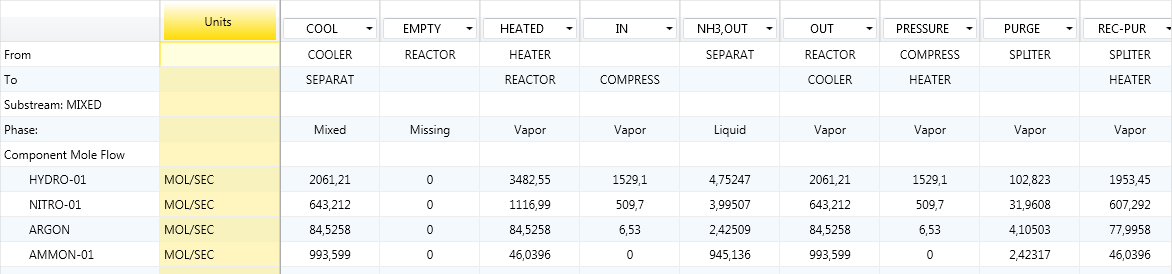
\includegraphics[scale=0.5]{RK-ASPEN.png}
	\end{center}
	\caption{Modèle \texttt{RK-ASPEN}, $750\si{\kelvin}$, $270\si{\bar}$, 5\%}
	\label{fig:RK-ASPEN}
\end{figure}

\begin{figure}[h!]
	\begin{center}
		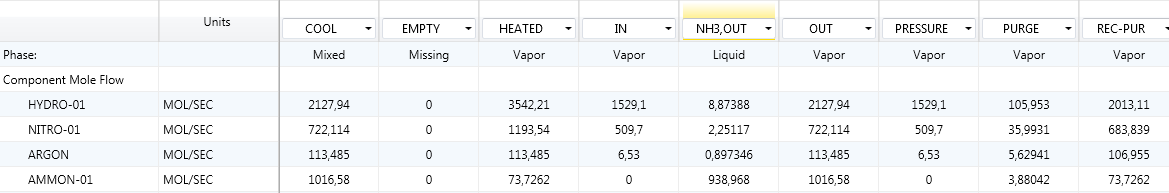
\includegraphics[scale=0.5]{PSRK.png}
	\end{center}
	\caption{Modèle \texttt{PSRK}, $750\si{\kelvin}$, $270\si{\bar}$, 5\%}
	\label{fig:PSRK}
\end{figure}

\begin{figure}[h!]
	\begin{center}
		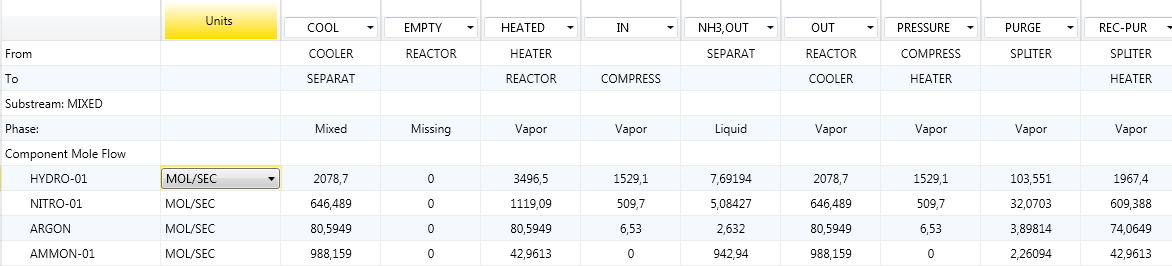
\includegraphics[scale=0.5]{SRK,750,270,5.png}
	\end{center}
	\caption{Modèle \texttt{SRK}, $750\si{\kelvin}$, $270\si{\bar}$, 5\%}
	\label{fig:SRK,750,270,0.05}
\end{figure}

\begin{figure}[h!]
	\begin{center}
		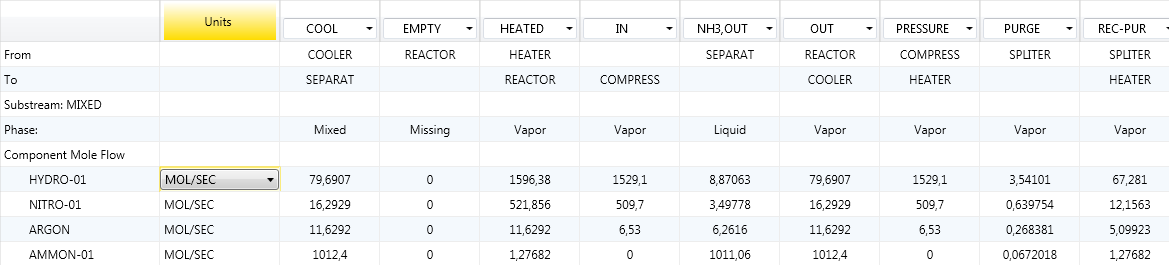
\includegraphics[scale=0.5]{SRK,500,270.png}
	\end{center}
	\caption{Modèle \texttt{SRK}, $500\si{\kelvin}$, $270\si{\bar}$, 5\%}
	\label{fig:SRK,500,270,0.05}
\end{figure}

\begin{figure}[h!]
	\begin{center}
		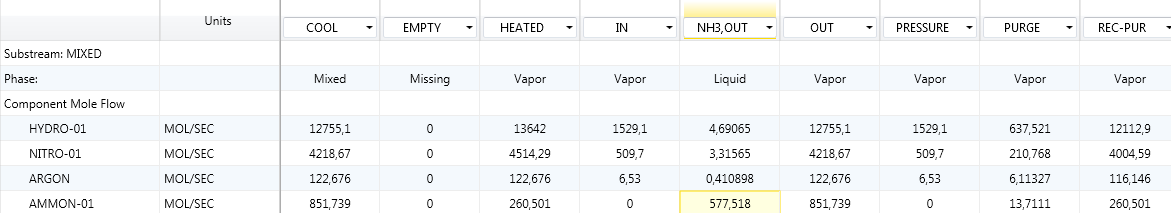
\includegraphics[scale=0.5]{SRK,1000,270.png}
	\end{center}
	\caption{Modèle \texttt{SRK}, $1000\si{\kelvin}$, $270\si{\bar}$, 5\%}
	\label{fig:SRK,1000,270,0.05}
\end{figure}

\begin{figure}[h!]
	\begin{center}
		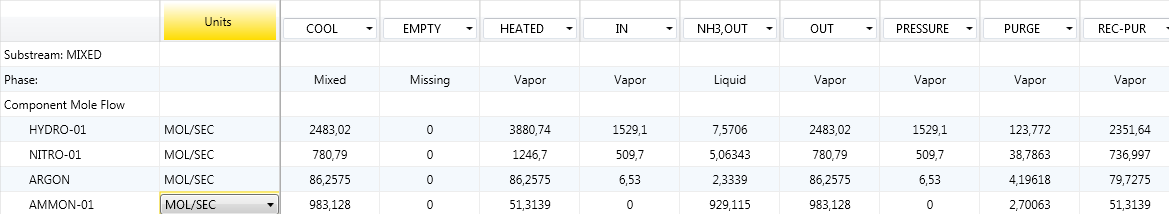
\includegraphics[scale=0.5]{SRK,750,220.png}
	\end{center}
	\caption{Modèle \texttt{SRK}, $750\si{\kelvin}$, $220\si{\bar}$, 5\%}
	\label{fig:SRK,750,220,0.05}
\end{figure}

\begin{figure}[h!]
	\begin{center}
		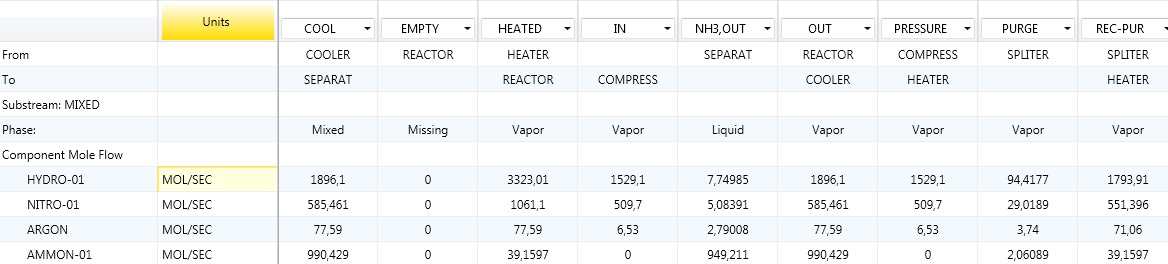
\includegraphics[scale=0.5]{SRK,750,300.png}
	\end{center}
	\caption{Modèle \texttt{SRK}, $750\si{\kelvin}$, $300\si{\bar}$, 5\%}
	\label{fig:SRK,750,300,0.05}
\end{figure}

\begin{figure}[h!]
	\begin{center}
		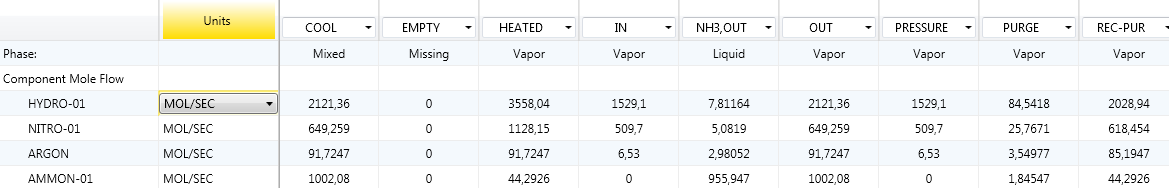
\includegraphics[scale=0.5]{SRK,750,270,4.png}
	\end{center}
	\caption{Modèle \texttt{SRK}, $750\si{\kelvin}$, $270\si{\bar}$, 4\%}
	\label{fig:SRK,750,270,0.04}
\end{figure}

\begin{figure}[h!]
	\begin{center}
		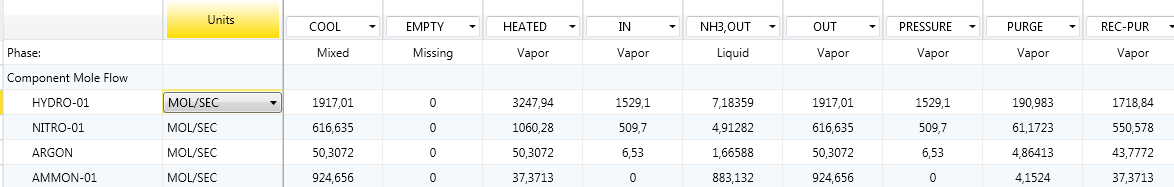
\includegraphics[scale=0.5]{SRK,750,270,10.png}
	\end{center}
	\caption{Modèle \texttt{SRK}, $750\si{\kelvin}$, $270\si{\bar}$, 10\%}
	\label{fig:SRK,750,270,0.1}
\end{figure}

\begin{figure}[h!]
	\begin{center}
		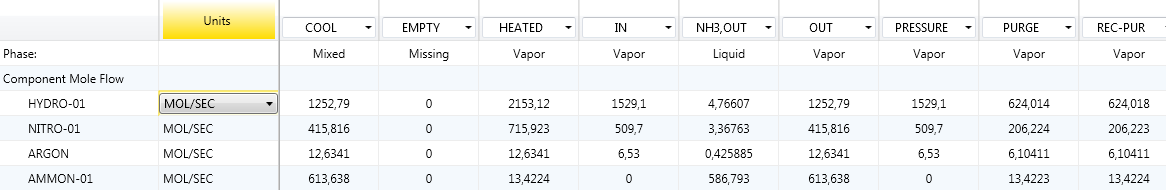
\includegraphics[scale=0.5]{SRK,750,270,50.png}
	\end{center}
	\caption{Modèle \texttt{SRK}, $750\si{\kelvin}$, $270\si{\bar}$, 50\%}
	\label{fig:SRK,750,270,0.5}
\end{figure}

\begin{figure}[h!]
	\begin{center}
		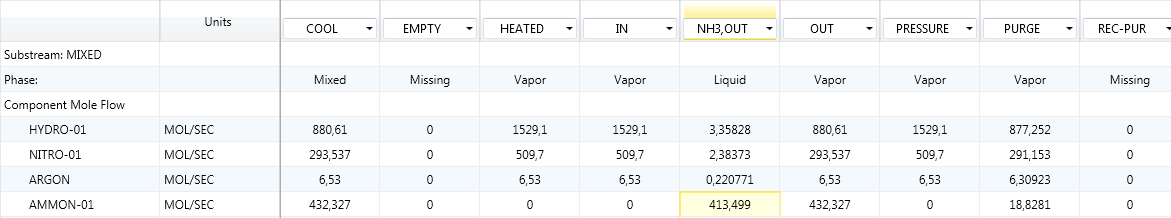
\includegraphics[scale=0.5]{SRK,750,270,100.png}
	\end{center}
	\caption{Modèle \texttt{SRK}, $750\si{\kelvin}$, $270\si{\bar}$, 100\%}
	\label{fig:SRK,750,270,1}
\end{figure}

\section{Outil de calcul: codes \textsc{Matlab}}




\printbibliography
\end{document}



\section{T\^ache 3}
% cedric

\section{T\^ache 4}
%\documentclass[a4paper,oneside,12pt]{article}

\NeedsTeXFormat{LaTeX2e}
\ProvidesPackage{custom}[2014/05/11 Custom Package]

\usepackage[utf8]{inputenc}
\usepackage[T1]{fontenc}
\usepackage[francais]{babel}

\usepackage[version=3]{mhchem}
\usepackage{chemfig}

\usepackage{amsmath}
\usepackage{amsthm}
\usepackage{amsfonts}

\usepackage{graphicx} 
\usepackage[top=3cm, bottom=3cm, left=3cm , right=3cm]{geometry}
%\usepackage{setspace} %doublespace, onehalfspace
\usepackage{siunitx}

\usepackage{tikz}
\usetikzlibrary{positioning}
\usetikzlibrary{shapes,arrows}

\usepackage{tabularx}
\usepackage{url} 
\usepackage{tocloft} %spacing in list of figures
\usepackage{listings} %input code
%\usepackage{multibbl} %multiplebibliography
\usepackage{hyperref}
\usepackage[babel=true]{csquotes}
\usepackage{listings}
\usepackage{color}

\usepackage{epstopdf}

\usepackage{caption}
\usepackage{subcaption}
\usepackage{float}

\newcommand{\dif}[1]{\mathrm{d}#1}
\newcommand{\e}[1]{\cdot 10^{#1}}

\endinput


\title{Tache 4 : Mini-\textsc{hazop} du noeud autour du réacteur de synthèse d'ammoniac}
\author{Groupe 1225}
\date{20 Novembre 2014}

\begin{document}

\maketitle

\section*{Question 1}

On retrouve $6$ gaz présents dans le réacteur. 
Certains ne présentent que peu de danger, 
d'autres peuvent provoquer d'importants dégats en cas de combustion.

\begin{itemize}	
	\item L'hydrogène est un gaz extrêmement inflammable et peut provoquer de grosses 
		explosions en cas de combustion. C'est le principal danger lié à sa présence. 
		En cas d'accumulation d'hydrogène dans une pièce ou un batiment, 
		sa présence peut provoquer un environnement déficient en oxygène et 
		donc provoquer la suffocation.

	\item  L'argon est présent naturellement dans l'air et n'est dangereux qu'en 
		quantités importantes. Il peut alors provoquer la suffocation.

	\item  L'azote est également naturellement présent dans l'air et n'est pas plus 
		dangereux que l'argon.

	\item  L'ammoniac est inflammable et peut donc provoquer une explosion en cas 
		d'accumulation et de combustion.

	\item  L'helium peut provoquer l'asphyxie en cas de concentration trop élevée.

	\item  Le méthane est inflammable et présente un danger d'explosion en cas 
		d'accumulation et de combustion. Il y a également un risque d'asphyxie en 
		cas d'accumulation simple.
\end{itemize}

\section*{Question 2}

Les PDF et PID se trouvent à la fin du rapport dans l'annexe \ref{ann:fluxes}.


\section*{Question 3}

\paragraph{1} Imaginons que pour une quelconque raison, il y ait une fuite de gaz inflammable, 
de l'hydrogène par exemple. Le gaz se propagerait alors dans l'atmosphère à 
une pression de $150\si{\bar}$ et à une température de $180\si{\celsius}$. 
Il s'enflammerait directement, créant ainsi une augmentation rapide de la température. 
Les canalisations, chauffées par les flammes, verraient leur pression interne augmenter 
brutalement. Les canalisations se déchireraient, entraînant la libération d'hydrogène 
supplémentaire, provoquant ainsi une déflagration.

Nous pourrions éviter le déchirement des canalisations en utilisant des disques de rupture 
au niveau de celles-ci. Si la pression interne dépasse un certain seuil, le disque de rupture 
se rompt, libérant le gaz, mais évitant la destruction des tuyauteries.

\paragraph{2} Prenons maintenant le cas où un problème survient au niveau du réacteur 
de synthèse de l'ammoniac. La réaction de synthèse

\begin{equation}
	\ce{\frac{3}{2} H2_{(g)} + \frac{1}{2} N2_{(g)} <=> NH3_{(g)}}
	\label{eq:synthesis}
\end{equation}

est une réaction exothermique ($-45.9\si{\kilo\joule}$ à $298\si{\kelvin}$). 
Elle dégage donc beaucoup de chaleur, qu'il faut traiter afin d'éviter 
une hausse trop importante de la température au sein du réacteur. 
En faisant circuler les gaz de synthèse \ce{H2 \, et \, N2},  
qui sont à $180\si{\celsius}$, dans les parois du réacteur, 
ceux-ci vont absorber une partie de la chaleur produite par la réaction. 
Nous nous apercevons donc que s'il y a une défaillance au niveau du système 
de refroidissement, par exemple si l'entrée des gaz de synthèse est bouchée, 
la température du réacteur va augmenter brusquement. Etant donné que le volume est fixe, 
la pression va augmenter proportionnellement à la température, 
jusqu'à ce qu'elle dépasse la limite supportable par les parois du réacteur. 
A ce moment-là, le réacteur explose sous l'effet de la pression.

Pour éviter cela, il faut construire le réacteur de manière à ce que 
le couvercle de celui-ci cède en premier en cas de surpression. 
Nous limitons de cette manière fortement les dommages occasionnés.

\paragraph{3} Etudions maintenant le cas d'un blackout électrique. 
L'installation est soudainement privée d'électricité. 
Les compresseurs vont donc s'arrêter, et l'apport en réactifs au niveau 
du réacteur va donc s'arrêter.
La réaction va continuer jusqu'à ce que les pressions au niveau des tuyauteries 
des réactifs et de l'ammoniac s'équilibrent.
La synthèse de l'ammoniac diminue la pression car elle réduit le nombre de moles 
de gaz présent, mais est exothermique, et puisque le refroidissement est effectué 
par les réactifs, et que le système n'est plus alimenté, le réacteur va chauffer.
Il va également falloir redémarrer le réacteur une fois l'élecricité rétablie. 
Le réacteur doit avoir le temps de refroidir afin d'éviter 
que la température ne soit trop élevée lors du redémarrage. 
Il sera cependant nécessaire de purger ou préchauffer le réacteur si
la température du réacteur est trop basse car la réaction ne se fera pas.

Nous pouvons éviter tout problème en ayant des générateurs sur site capable 
de délivrer de l'électricité en cas de blackout jusqu'à ce que 
le courant soit rétablit. 

\section*{Question 4}
% Pourquoi n’y a-t-il pas de soupape de sécurité ou de disque de rupture (les deux types 
% de dispositifs servent à protéger un équipement ou une ligne contre les surpressions) 
% sur le réacteur de synthèse du NH3 ?

Un disque de rupture est un dispositif de sécurité qui sert à protéger les installations 
contre les surpressions.
La réaction de synthèse de l'ammoniac est la réaction \ref{eq:synthesis}.
On remarque immédiatement qu'il y a une diminution du nombre de moles de gaz (d'un facteur 2) 
lorsque de l'ammoniac est produit. La loi des gazs parfait nous indique que la pression
exercée par un gaz est directement proportionnelle à son nombre de moles.
Une surpression n'est pas envisageable pour cette réaction, 
il n'y a donc pas besoin de disque de rupture sur ce réacteur.

\section*{Question 5}
% Pourquoi y a-t-il des disques de rupture sur l’échangeur 124-MC ?

L'échangeur 124-C est un dispositif permettant de transférer de la chaleur d'un fluide
vers un autre, sans que ceux-ci ne se mélangent.
On a donc un flux \emph{chaud} et un flux \emph{froid}. Le flux froid va recevoir de 
l'énergie thermique et sa température va augmenter, il faut alors prévoir des disques 
de rupture au cas où la température dépasse une certaine limite qui produirait une 
supression du gaz et pourrait endommager, voire déchirer, la paroi.
Théoriquement, le flux chaud n'a pas besoin de disque de rupture parce que le gaz qu'il 
transporte ne peut que diminuer de volume. Cependant, on peut toujours considérer le cas
d'un apport soudain et imprévu de chaleur comme une explosion extérieure, qui produirait
une augmentation de température et par conséquent de pression. 
Il devient alors nécessaire d'avoir des disques de rupture dans les deux sens de l'échangeur.


\appendix
\section{Circulation des flux de matières - PDF et PIDs}
\label{ann:fluxes}

\begin{center}
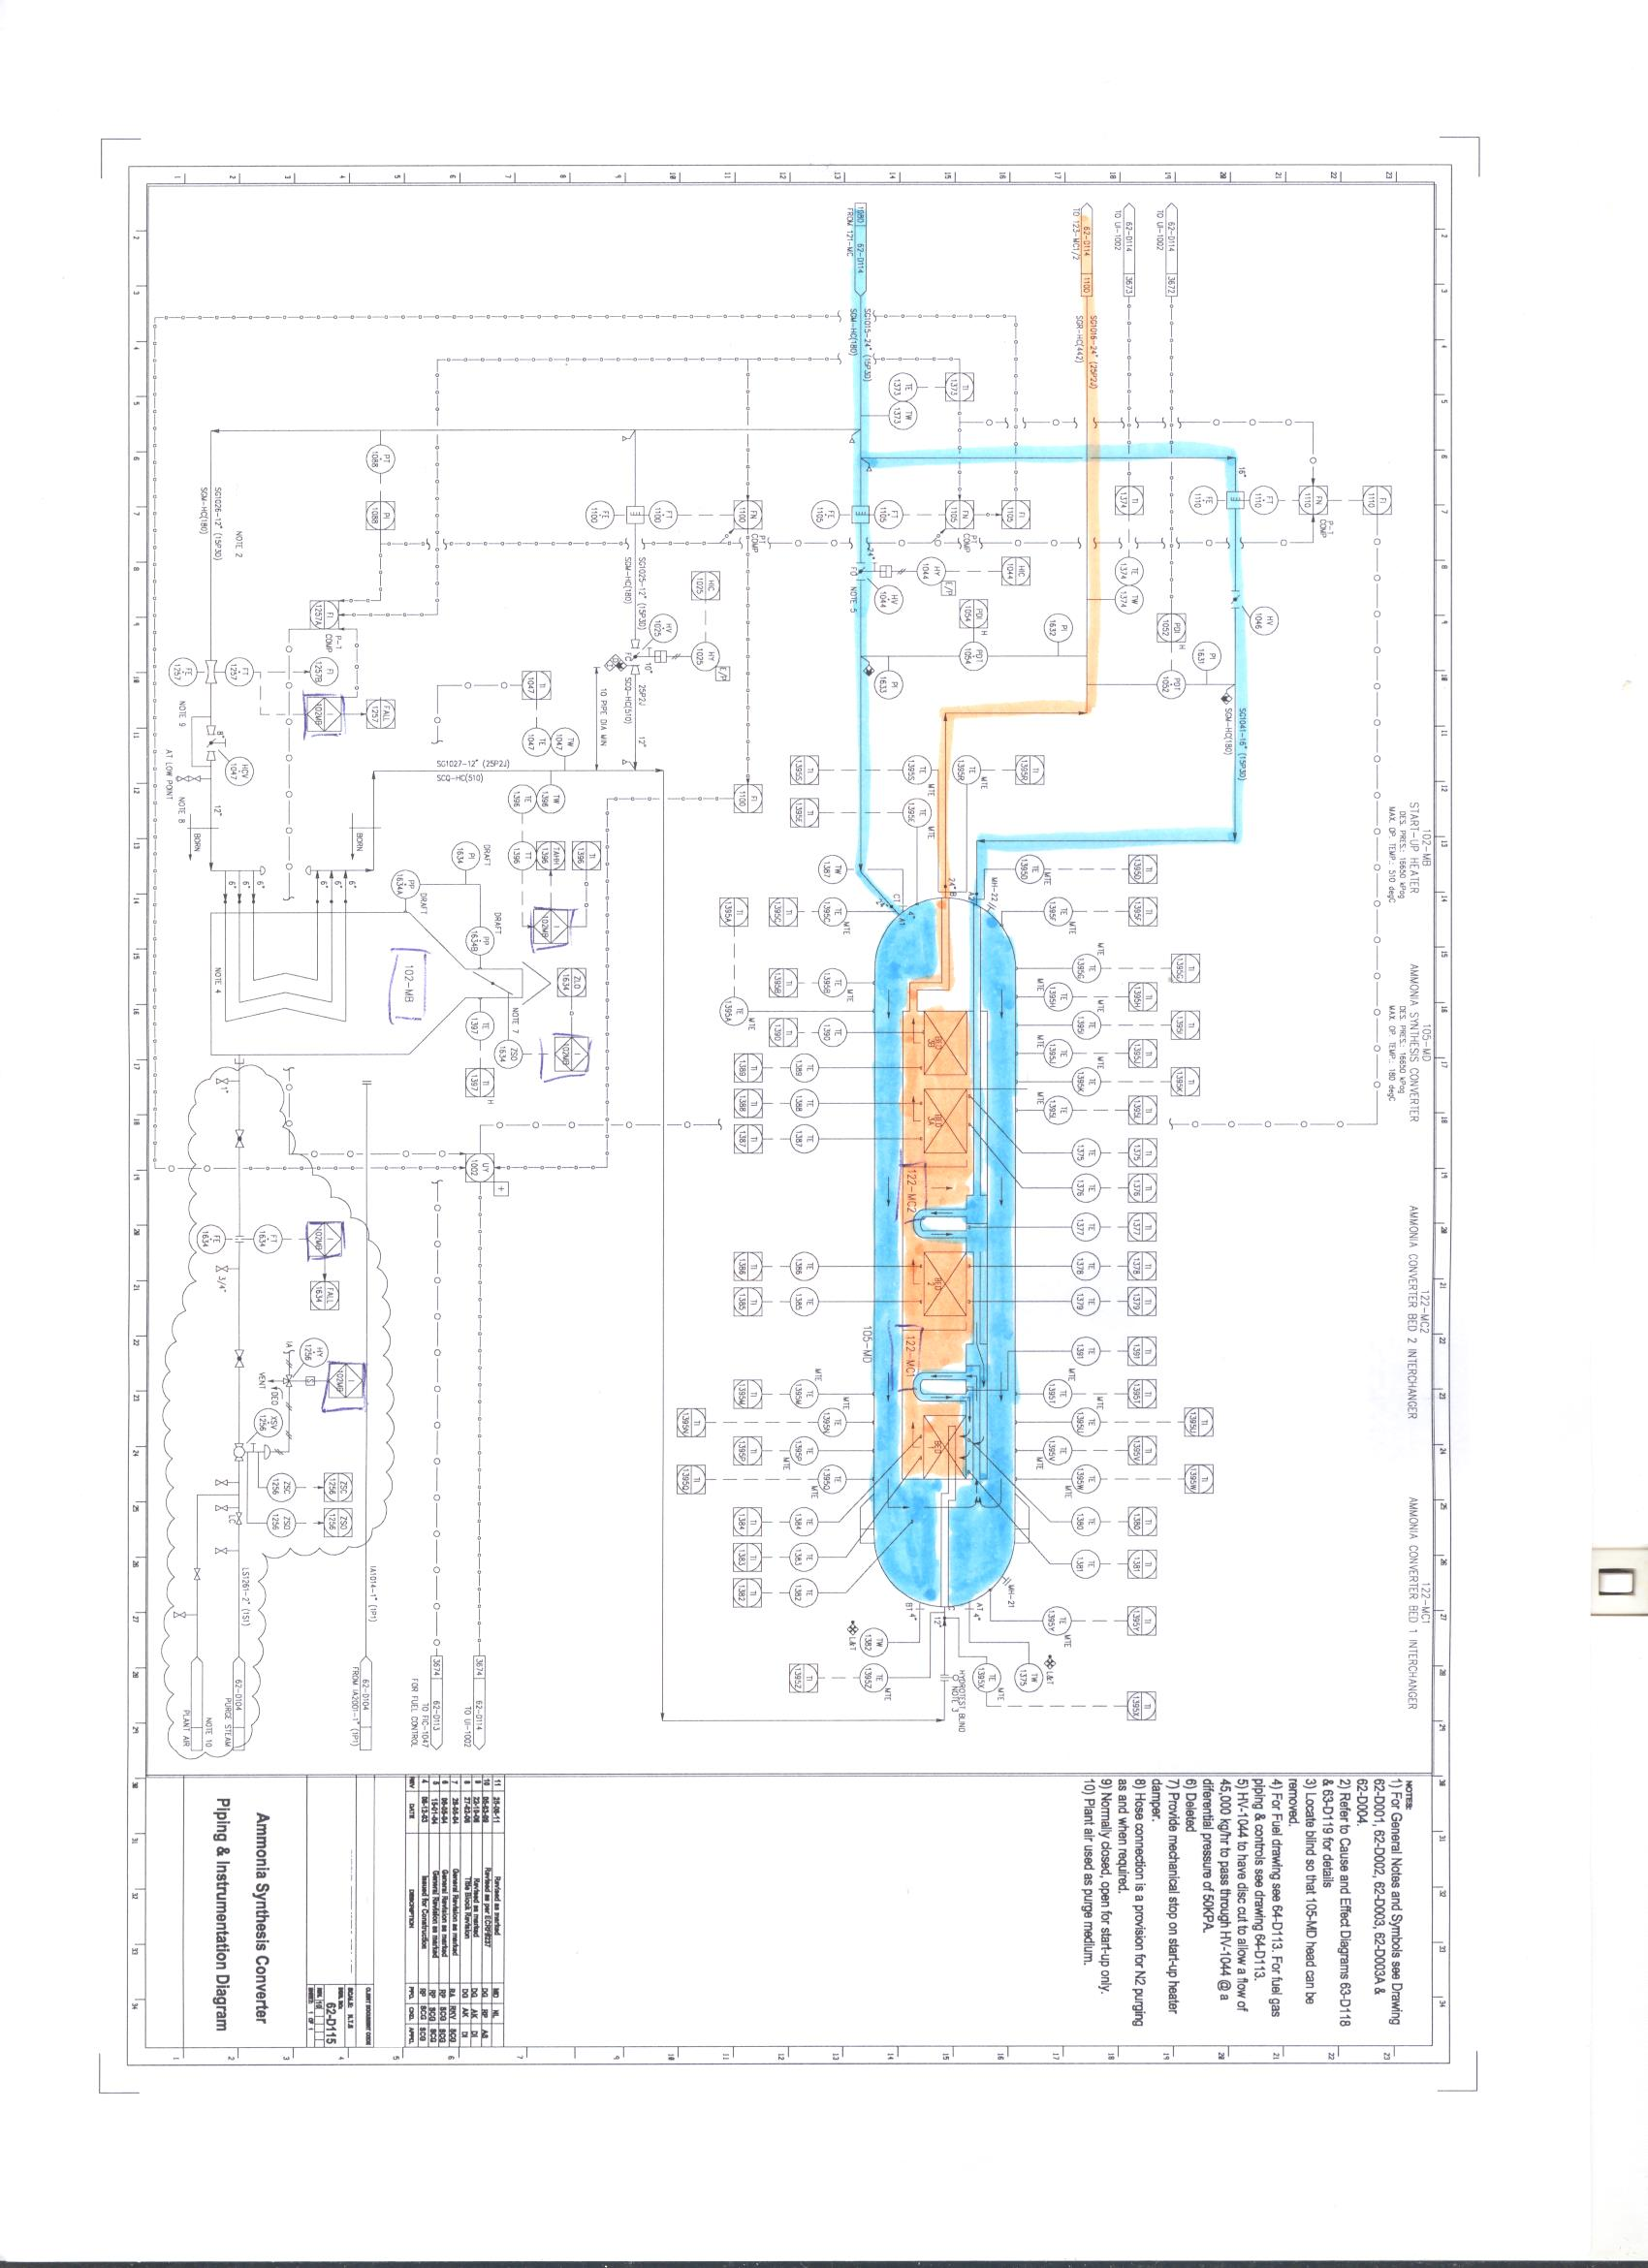
\includegraphics[scale=0.7]{001.jpg}

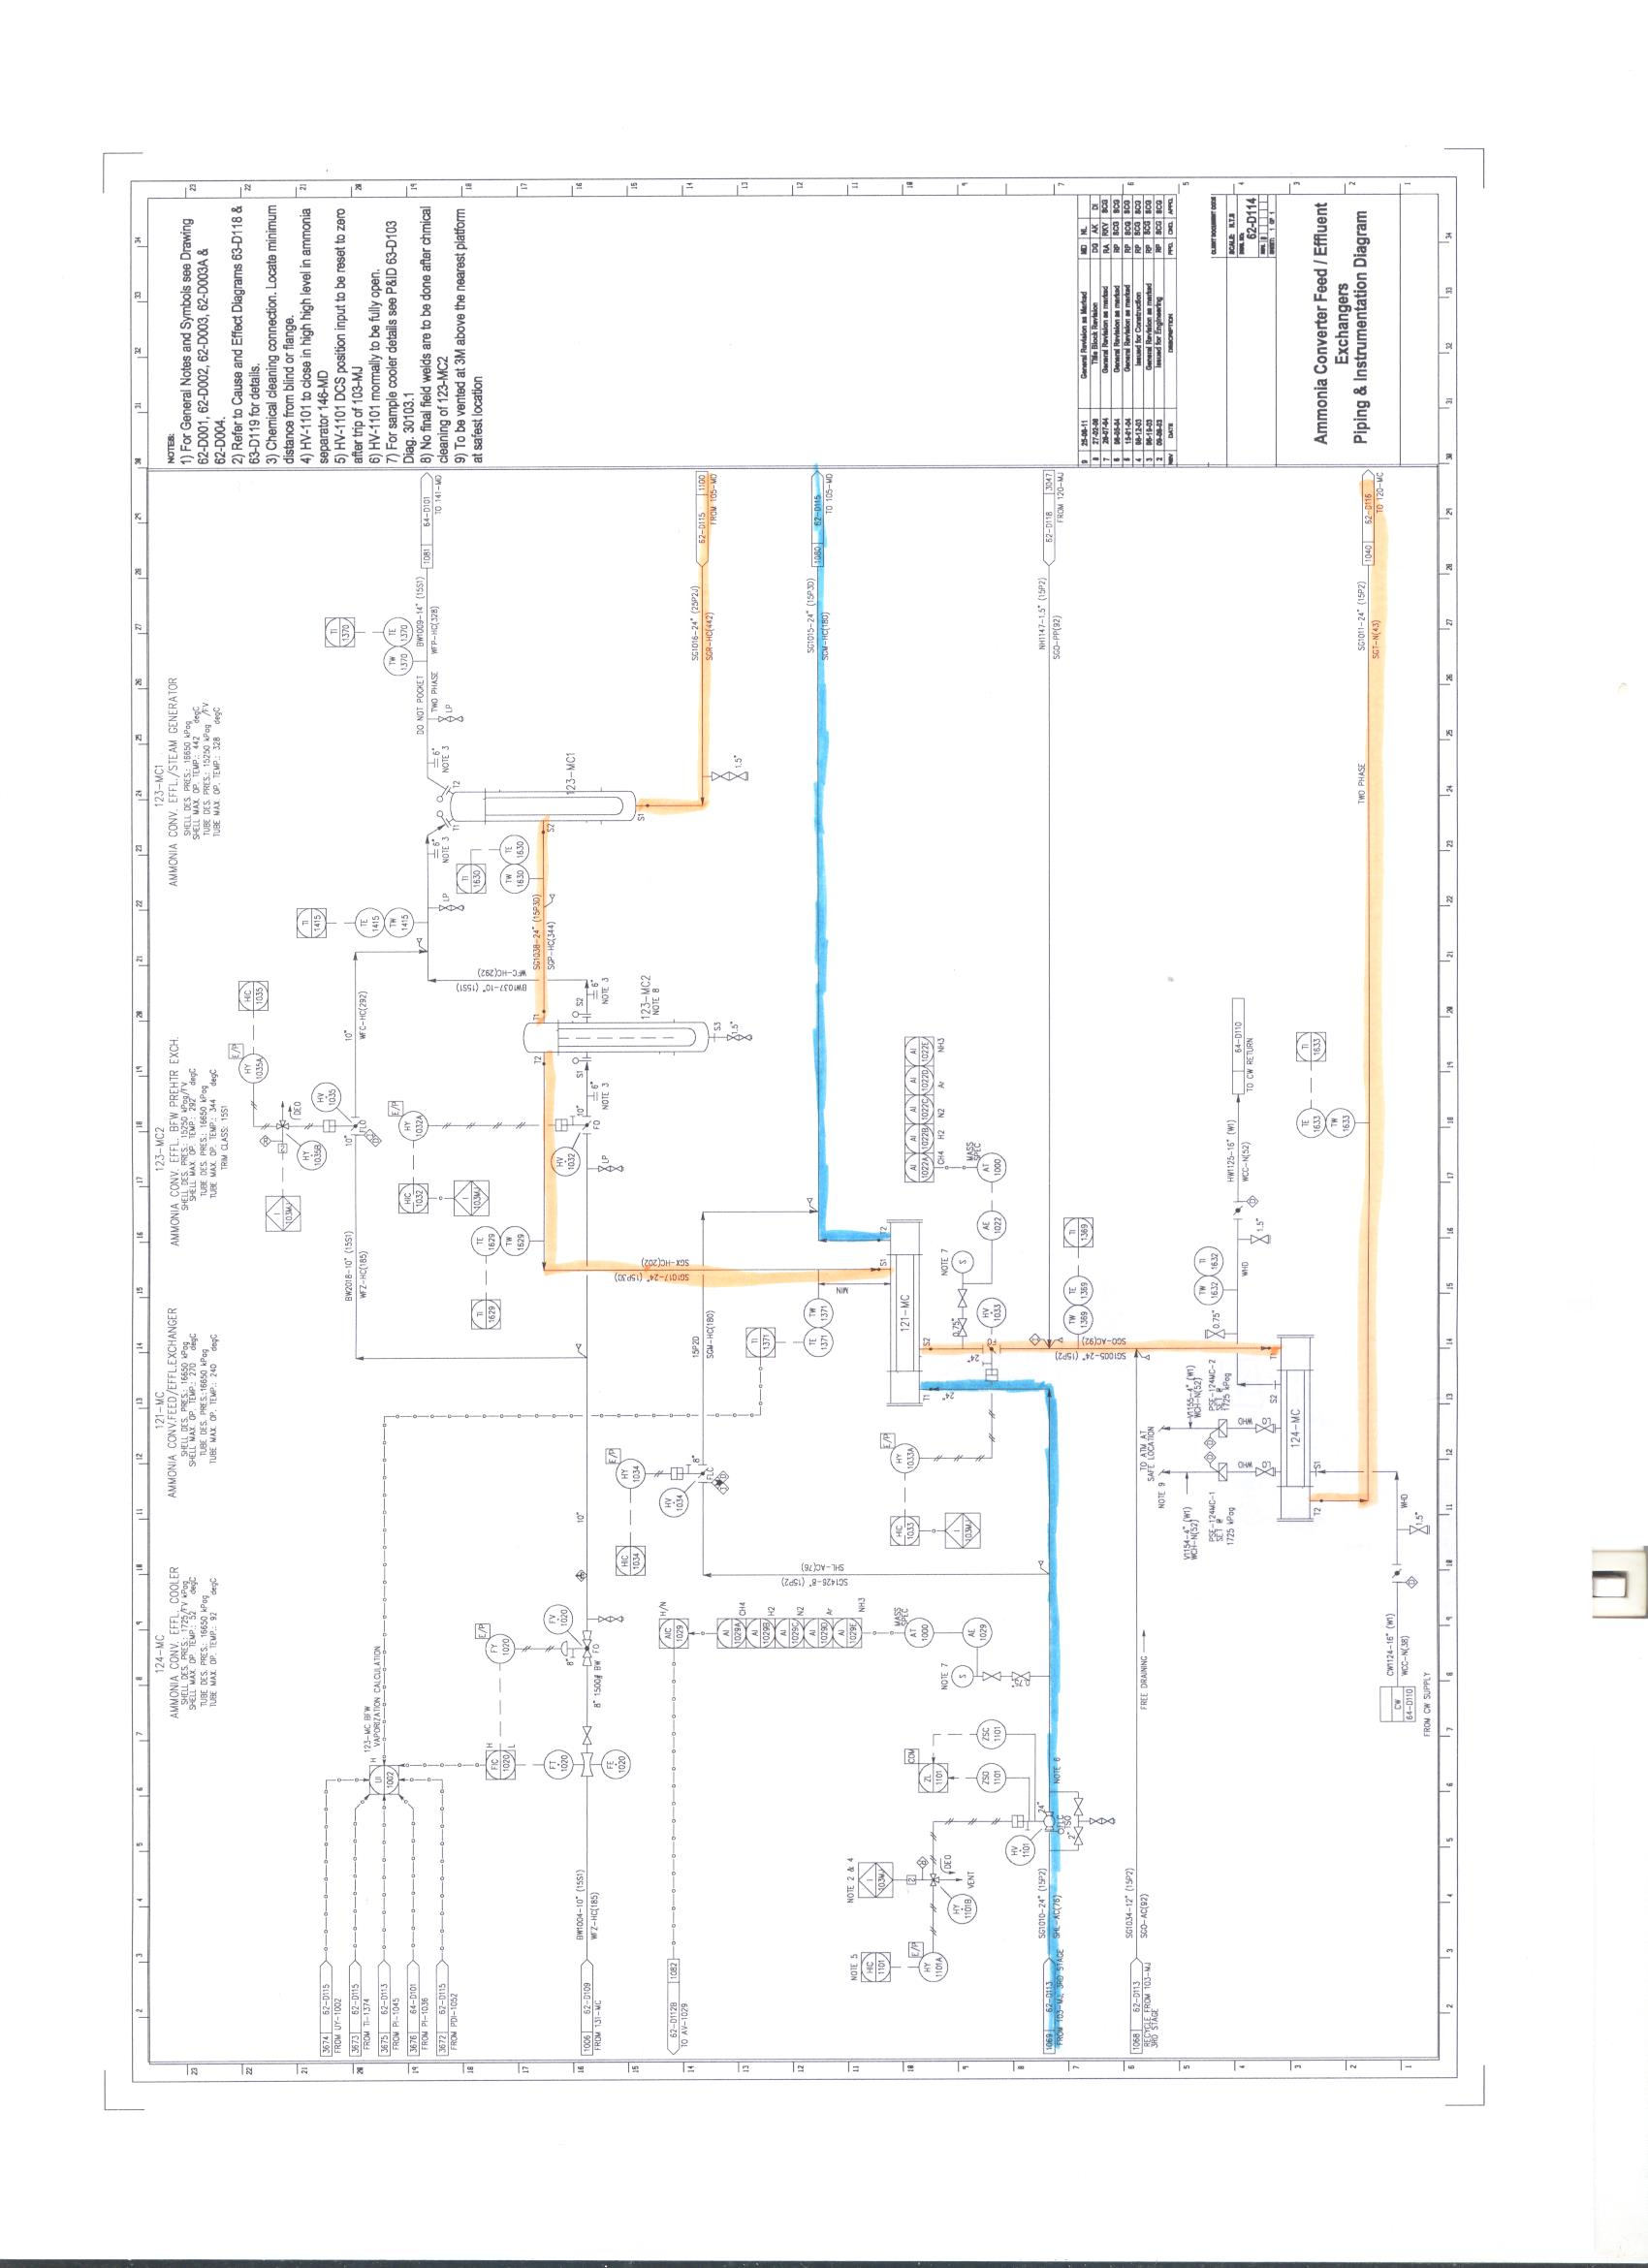
\includegraphics[scale=0.7]{002.jpg}

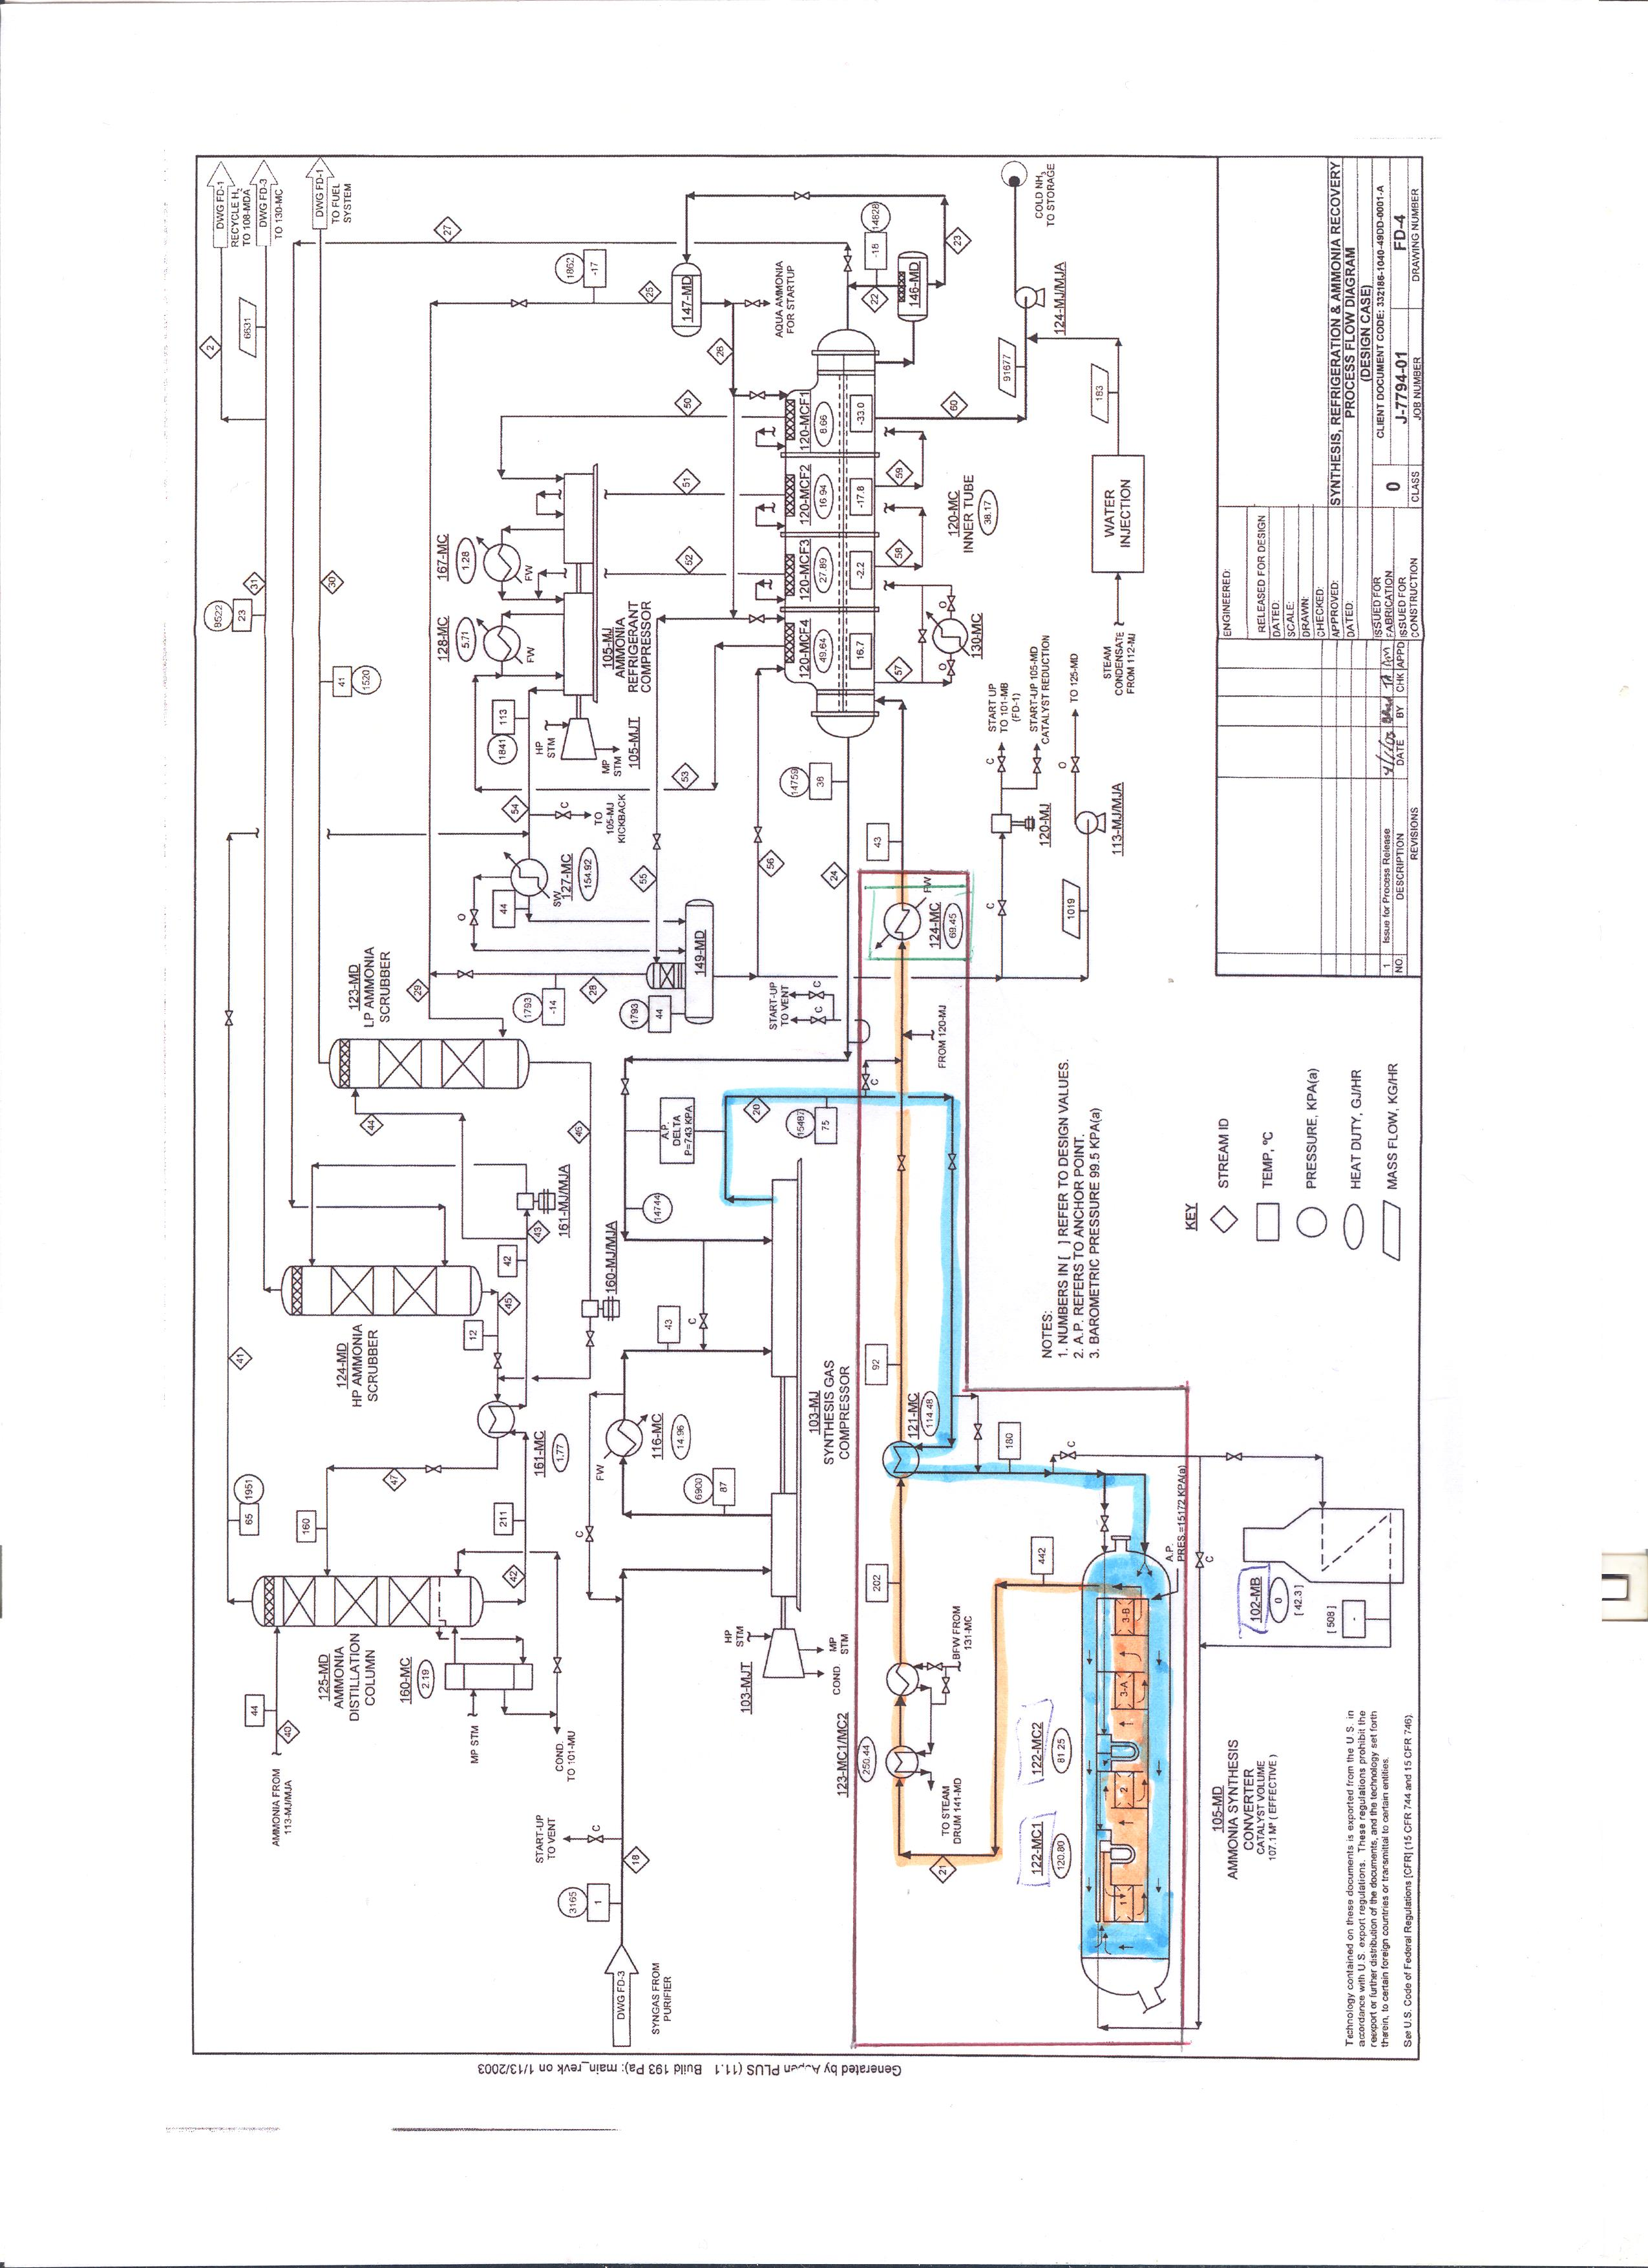
\includegraphics[scale=0.7]{003.jpg}
\end{center}

\end{document}


\section{T\^ache 5}
%Pour la t\^ache 5, il nous était demandé de dimensionner une soupape de sécurité
pour un tank contenant de l'ammoniac. Pour celà, nous avons recu quelques informations:

\begin{itemize}

\item Forme du tank: cylindrique vertical à extrémités hémisphériques. Tank au sol.
\item Hauteur totale du tank: $12 \si{\metre}$
\item Niveau de \ce{NH3} liquide dans le tank: $8\si{\metre}$
\item Diamètre du tank: $6 \si{\metre}$
\item Température normale de stockage: $20 \si{\degreeCelsius}$
\item Pression de design: $15 \barg$
\item Cp/Cv du \ce{NH3}: $1.33$; Facteur de compressibilité Z: $1.0$
\item La soupape sera une soupape conventionnelle et la contrepression sera nulle.
\item L’usine est munie de systèmes de drainages des fuites 
	et d’un équipement moderne de lutte contre l’incendie.
\end{itemize}

Nous avons également à notre disposition deux graphes donnant respectivement 
les pressions de stockage de l'ammoniac et de l'enthalpie de vaporisation 
en fonction de la température.

\paragraph{Remarque}
A travers cette section nous utilisons l'unité \barg, 
qui correspond à la pression supérieur à la pression atmosphérique.
On a donc:
\[ p [\barg] = p [\si{\bar}] - 1 \]

% Quelle est la pression normale de stockage ?
\section{Pression normale de stockage} 
La pression normale de stockage est de $7.8 \barg$ à $20\si{\celsius}$ 
(température normale de stockage). Nous avons obtenu ces résultats sur base des
graphiques que nous avions reçus.

% Quelle sera la pression de stockage en été (30°C) ?
\section{Pression de stockage en été} 
La pression de stockage en été est de $10.625 \barg$ à $30\si{\celsius}$.

% Quel sera la pression maximale de tarage de la soupape de sécurité ?
\section{Pression maximale de tarage de la soupape} 
La pression maximale de tarage de la soupape de sécurité vaut 
\[ 121\% \cdot p_{\text{design}} = 18.15 \barg \]

% Dimensionner la soupape pour cette pression de tarage.
%     -	Quelle sera la pression durant la décharge ?
%     -	Quelle sera la température du liquide durant la décharge via la soupape ?
%     -	Quelle sera la taille de la soupape nécessaire ?
\section{Dimensionnement de la soupape} 
La pression durant la décharge sera de $19.16325 \si{\bar}$. 
Cette pression est fort élevée car nous considérons le cas d'un incendie au niveau du réservoir. 
La température du gaz durant la décharge sera de $50\si{\celsius}$. 
Nous aurons besoin d'une soupape d'une section de $730\si{\milli\meter\squared}$ 
ou $1.13 \, \text{inch}^2$. Ceci correspond à une PSV de type $2J3$
\[ C = 0.03948 \cdot \sqrt{1.33 \cdot \frac{2}{2.33}^{\frac{2.33}{0.33}}} \]
\[ W = 43200 \cdot 1 \cdot 143.634^{0.82} \]
\[ A = \frac{W}{C \cdot 0.975 \cdot 20.071 \cdot 1 \cdot 1} \cdot \sqrt{\frac{323.15}{17}} \]

\section{Effet de l'augmentation de la pression de tarage de 5 à 20 barg pour une pression de design de 20 barg} 
Si la pression de design est à $20\barg$, nous pouvons augmenter la pression de tarage à \[ 121\% \cdot p_{\text{design}} = 24.2\barg \]

Nous recalculons A avec la pression et température plus élevées,
et obtenons que la soupape doit avoir une section de $590\si{\milli\meter\squared}$
ce qui nous donne $0.9118 \, \text{inch}^2$. Ceci correspond à une PSV de type $2J3$ comme celle trouvée précédemment. Il n'y a donc pas d'intérêt
à augmenter la pression de design dans ces conditions.

% Pour la première pression de tarage, quelle est l’influence d’isoler thermiquement 
% le tank avec un isolant tel que le coefficient d’échange avec l’extérieur 
% soit réduit à une valeur de 10 W/m2.K ? 
\section{Isolation thermique du tank}
Nous isolons la cuve avec un isolant réduisant le coefficient d'échange de la cuve avec l'extérieur à 
$10 \si{\watt}/\si{\meter\squared} \cdot \si{\kelvin}$
On réduit donc le facteur environnemental à $F = 0.15$. 
Notre $W$ va donc être fortement réduit, et nous pouvons donc réduire la taille de la soupape à 
$110\si{\milli\meter\squared}$ ou $0.17 \, \text{inch}^2$. 
Cette PSV est du type $1E2$. L'ajout de l'isolant réduit donc fortement la taille de
la soupape requise.



\section{T\^ache 7}
%\documentclass[a4paper, oneside, 12pt]{article}

\usepackage{../custom}

\title{Rapport des activités de terrain}
\author{Groupe 1225}
\date{12 Novembre 2014}

\begin{document}

\maketitle

\section{Visite de la station de biométhanisation de l’AIVE à Tenneville}

L’usine de biométhanisation permet de créer du CH4 à partir de déchets organiques,
principalement ménagers, mais aussi provenant de parcs à container, etc.

Premièrement, les déchets sont acheminés par camions au centre de Tenneville.
Avant d’être stocké dans un entrepôt, les camions passent à travers un portique afin 
de détecter s’il y a une présence de déchets radioactifs, ils sont ensuite pesés
puis sont déchargés dans le premier entrepôt.

Les déchets passent à travers un broyeur et sont acheminés par tapis roulant 
ou des aimants permettent d’y retirer les déchets ferreux indésirables.
À cette étape, les déchets sont prêts à entrer dans le digesteur. 
Ce digesteur ressemble à un grand silo d’une capacité de $3000 \si{\meter\cubed}$.
Le principe est assez simple, des bactéries anaérobies vont commencer à digérer 
ces matières organiques en l’absence d’oxygène, ce qui crée du méthane. 
Le méthane sert à la production d’électricité et de chaleur (principe de cogénération).
L’usine est donc indépendante en électricité et en chauffage.
L’excédent  d’électricité est redistribué sur le réseau, et l’excédent de chaleur 
est utilisé au séchage de boue ainsi qu’a d’autres usines de recyclages. 

Une fois la matière digérée, elle est compostée complètement jusqu’à l’obtention 
de terreau qui est revendu aux agriculteurs.
En cas de panne de moteur, ou tout autre problème dans le digesteur,
il y a une torchère qui permet du brûler tout excédent de méthane
et donc éviter tout surplus dans le digesteur, cela évite aussi de devoir 
libérer du méthane dans l’atmosphère.

Quelques chiffres :
\begin{itemize}
	\item Capacité de traitement : $39 000$ tonnes par an
	\item Production en électricité : équivalent à la consommation de $1500$ ménages
	\item Production de gaz : $55\%$ de \ce{CH4}, $44\%$ de \ce{CO2} + autres gaz
\end{itemize}

\section{Visite du centre Total Research Technology Feluy}

\subsection{Catalyse}
 
L'utilisation d'un catalyseur est essentielle pour de nombreuses réactions industrielles 
effectuées aujourd'hui. De nombreuses réactions ne seraient même pas possibles sans 
l'utilisation d'un catalyseur.
 
Un catalyseur réduit l'énergie d'activation d'une réaction en affaiblissant les liens
électroniques des molécules devant réagir, ou en affaiblissant les liens entre les 
molécules des réactifs. Certains catalyseurs sont en pratique ``consommés'' durant 
la réaction (ex: emprisonnés dans les molécules) et d'autres ne sont simplement pas 
affectés par les réactions. 

Dans de nombreuses réactions, les catalyseurs ont également d'autres rôles. 
Suivant le catalyseur utilisé, certaines réactions seront favorisées au détriment 
d'autres (il faut donc trouver un catalyseur favorisant la réaction voulue). 
Le catalyseur peut également déterminer la structure des molécules obtenues lors 
d'une cristallisation. Suivant le catalyseur utilisé lors de la synthèse de polyéthylène,
on obtiendra une poudre fine ou de plus gros grains,
deux structures ayant des applications différentes.
 
Trouver le bon catalyseur est donc essentiel dans la chimie moderne.
 
\subsection{Unités Piliotes}
 
Le développement de nouveaux procédés ou catalyseurs commence tout d'abord en laboratoire,
ou de microréacteurs permettent de tester la viabilité des nouveaux développements.
Si un catalyseur ou un procédé est considéré comme intéressant,
il va ensuite être testé dans une unité pilote. 

Différentes réactions demandent différents réacteurs,
et le réacteur idéal pour une nouvelle réaction est déterminé en laboratoire.
 
Les unités pilotes sont des réacteurs industriels réduits utilisés pour tester de
nouvelles réactions ou de nouveaux procédés. Les unités pilotes sont beaucoup plus
modulables que les unités industrielles. Celles-ci vont permettre de détecter
d'éventuels problèmes qui sont passés inaperçus lors des tests en laboratoires,
ainsi que de déterminer les conditions idéales pour l'utilisation des nouvelles réactions.
Si un nouveau produit (nouvelle structure ou autre) est considéré comme intéressant,
les unités pilotes vont permettre de produire une quantité limitée de ce nouveau
produit afin de fournir des échantillons à des partenaires commerciaux.
Elles évitent ainsi de devoir reconfigurer des plants de grande taille.

\section{Laboratoire d’électrolyse}

L'électrolyse de l'eau est un procédé qui permet de décomposer celle-ci en dioxygène 
et en dihydroègne, tous deux à l'état gazeux.

\begin{equation*}
	\ce{H2O_{(g)} \rightleftharpoons \frac{1}{2} \, O2_{(g)} + H2_{(g)}} 
\end{equation*}

Afin de produire du dihydrogène gazeux en quantités décentes, l'électrolyse de l'eau 
demande énormément d'énergie électrique (sous forme de courant). De plus, le rendement
de la réaction d'électrolyse de l'eau ne dépasse en général jamais les $50\%$, 
et améliorer celui-ci demanderait une trop grande tension électrique.

Sur base des expérimentations effectuées en laboratoire, nous observons que plus 
le milieu de la réaction est acide plus son degré d'avancement augmente. Il est donc
préférable de réaliser cette réaction dans un milieu où le pH est proche de zéro.


\begin{equation*}
	It = \text{constante}
\end{equation*}

où I est l'intensité du courant électrique, et t, le temps écoulé.
Cela dit bien que lorsqu'on augmente le courant, le temps diminue dans un rapport identique.

Si nous devions produire le dihydrogène dont nous avons besoin en utilisant la 
réaction d'électrolyse de l'eau, il faudrait tout d'abord veiller à ce que le pH soit le
plus faible possible. Ensuite, nous devrions calculer l'intensité du courant nécessaire
pour obtenir le débit de dihydrogène voulu.

Par exemple, si nous voulons une production de $1500 \si{\tonne}$ d'ammoniac par 
jour (en prenant une température de $1000 \si{\kelvin}$ pour le reformeur primaire),
nous savons grâce à notre outil de calcul qu'il faut $266,32 \si{\tonne}$ de dihydrogène
par jour. Cela nous donne un débit massique de $184,944 \, \si{\kilo\gram/\minute}$.

Ensuite, à l'aide des résultats obtenus lors du laboratoire, nous savons qu'avec 
un courant de $1 \si{\ampere}$, nous produisons $8 \, \si{\milli\liter}$ de dihydrogène
par minute. Considérons maintenant que le dihydrogène se comporte comme un gaz parfait,
nous pouvons appliquer :

\begin{equation*}
	pV = mR^{*}T
\end{equation*}

et donc caluler la masse de dihydrogène, sachant que la réaction se déroule sous 
des conditons standards de température ($298,15 \si{\kelvin}$) et de pression ($1 \si{\bar}$).
Nous obtenons ainsi qu'en faisant circuler un courant de $1 \si{\ampere}$,
nous produisons $6,4547.10^{-7} \, \si{\kilo\gram/\minute}$ de dihydrogène.

Pour atteindre un débit massique de $184,944 \, \si{\kilo\gram/\minute}$,
il faut donc un courant électrique de $2,865.10^8 \si{\ampere}$. À partir de la résistance
totale du système au sein duquel se déroule la réaction d'électrolyse,
qui est de $14 \, \si{\ohm}$, nous pouvons calculer la puissance électrique nécessaire : 

\begin{equation*}
	P = RI^{2}
\end{equation*}

Elle est donc égale à $1,15 \, \si{\giga\watt}$.

Nous remarquons effectivement que l'électrolyse de l'eau demande beaucoup trop d'énergie
pour produire ce dont nous avons besoin. C'est pour cela que l'électrolyse est très peu 
utilisée à l'échelle industrielle. Il est donc préférable dans notre cas de se contenter
du vaporeformage, malgré le fait qu'il émette du dioxyde de carbone.

\section{Visite du plant de Yara à Tertre}

\section{Atelier créatif (conduite de brainstorming)}

Comment faire preuve d'inventivité et d'originalité dans un projet tel que le nôtre ?
Tel était le thème de cet atelier où l'on nous a présenté le cheminement 
à suivre afin de mettre un maximum à profit la créativité de chacun.

Dans notre cas, la créativité est avant tout l'art de trouver des solutions 
originales et efficaces à un problème bien posé. 
La première partie du travail consiste donc à reformuler la problématique de façon 
à être capable de diverger et de trouver un angle nouveau sous lequel analyser le problème. 
Pour cela, il est conseillé de faire un schéma sur lequel on pourra retrouver différents
éléments comme par exemple les services attendus, la position géographique, 
ce qui se situe à proximité de l’usine,etc.

Cette représentation permet d'avoir une vue d'ensemble sur le travail qui 
devra être effectué et facilite donc l'organisation. Il est important de pousser tout
le monde à sortir de sa ``zone de confort'' et de confronter les idées de chacun.
Vient ensuite le retour à la réalité: il faut analyser les idées, choisir celles qui 
sont réalisables pour que le projet se précise enfin. De nombreux exercices ont été 
proposés afin de nous mettre en situation. 

Nous pouvons à présent faire bénéficier le reste du groupe de notre expérience et tenter
de suivre cette approche. Il est nécessaire de faire un résumé de tout cela pour essayer 
de convaincre et de prouver la viabilité de l'ébauche. Pour cela, on fait la liste 
de quatre choses: les besoins du client, la promesse, les raisons d'y croire, 
et un slogan pour accrocher. On continue l'argumentation avec des analogies,
des choses factuelles (brevets,...) ou inspirantes, etc. Le projet pourra alors
enfin être mis en place!

Une présentation sur le développement durable a aussi été faite afin de nous sensibiliser
et nous inviter à essayer d'y participer. 
En effet, notre système industriel actuel - où la recherche du profit occupe une position
centrale - est voué à l'échec, car il mène à des crises dans de nombreux domaines.
C'est pourquoi la société doit se remettre en question et évoluer pour atteindre
l'idéal d'un système organique, où l'humanité travaillerait ensemble pour un but commun. 

Dans notre cas, cela se résume à se préoccuper de l'écologie mais pas uniquement:
il serait intéressant de collaborer avec d'autres sociétés au niveau de l'importation
des ressources et de l'exportation nos déchets. Ces derniers pourraient être utiles
à d'autres et nous pourrions ainsi trouver des ententes profitables pour tous,
s'approchant d'un système cyclique.

\end{document}



\section{T\^ache 8}
%\documentclass[a4paper, oneside, 12pt]{article}

\usepackage{../custom}

\title{Tâche 8}
\author{Groupe 1225}
\date{3 Décembre 2014}

\begin{document}

\maketitle

\chapter{Enjeux environnementaux liés à la production d'ammoniac}



\end{document}



\chapter{Outil de gestion}
%\documentclass[a4paper,oneside,11pt]{article}

\usepackage{../../custom}

\title{\textsc{readme} de l'outil de gestion}
\author{Groupe 1225}
\date{\today}

\newcommand{\fun}[1]{\texttt{#1}}

\begin{document}

\maketitle

\section{Utilisation}

Lancer la fonction \fun{startOutil}.

\paragraph{Remarque} Il se peut que pour certaines valeurs de $m_\ce{NH3}$,
une erreur de type ``\textit{Could not extract individual solutions. 
Returning a MuPAD set object.}'' survienne lors de l'appel à \fun{main}. 
Pour palier à ce problème il suffit de changer la valeur 
de $m_\ce{NH3}$ d'une unité.

\section{Fonctionnement}

Voici une liste de l'ensemble des fonctions utilisées dans notre 
outil de gestion.

\begin{itemize}
	\item \fun{airePSV}
	\item \fun{analyseParametrique}
	\item \fun{environnement}
	\item \fun{getCoefficients} 
	\item \fun{getDeltaH\_and\_S}
	\item \fun{getEqConstantsRef} 
	\item \fun{getHovenMasses}
	\item \fun{getMassesDetails}
	\item \fun{getMolarMasses}
	\item \fun{getTubesNumber}
	\item \fun{main}
	\item \fun{printHovenDetails}
	\item \fun{printMassesDetails}
	\item \fun{purge}
	\item \fun{purgeP}
	\item \fun{purgeT}
	\item \fun{refroidissement}
	\item \fun{simulation}
	\item \fun{solveG}
	\item \fun{startOutil}
\end{itemize}


\paragraph{Limite de validité}
Les coefficients utilisés dans les équations de Shomate ne sont 
cependant valables que pour une certaine gamme de températures 
(on retrouve les températures acceptables pour chaque composé 
en commentaire dans le fichier \fun{getCoefficients}). 
On peut donc s'attendre à une certaine erreur sur les résultats 
si l'utilisateur entre une température non réaliste. 

Afin de palier à ce soucis, nous avons créé une fonction \fun{myAssert}. 
Celle-ci est une variante de la fonction \fun{Assert} 
et permet d'afficher un message d'avertissement, 
tout en continuant l'éxécution du programme.


\end{document}

\chapter{Aspen +}

\chapter{Support de présentation}


\printbibliography
\end{document}

